%===================================================================================
\section{Forward sensitivity analysis example problems}\label{s:fwd_ex}
%===================================================================================

For all the {\cvodes} examples, any of three sensitivity method options
(\id{CV\_SIMULTANEOUS}, \\
\id{CV\_STAGGERED}, or \id{CV\_STAGGERED1}) can be used, and sensitivities may be 
included in the error test or not (error control set on \id{TRUE} or \id{FALSE},
respectively).

The next three sections describe in detail two serial examples
(\id{cvsAdvDiff\_FSA\_non} and \id{cvsRoberts\_FSA\_dns}), 
and a parallel one (\id{cvsDiurnal\_FSA\_kry\_p}).
For details on the other examples, the reader is directed to the comments in
their source files.

%--------------------------------------------------------------------
\subsection{A serial nonstiff example: cvsAdvDiff\_FSA\_non}
\label{ss:cvsAdvDiff_FSA_non}

As a first example of using {\cvodes} for forward sensitivity analysis,
we treat the simple advection-diffusion equation
for $u=u(t,x)$
\begin{equation}\label{e:cvsAdvDiff_FSA_non_PDE}
  \frac{\partial u}{\partial t}= q_1 \frac{\partial ^{2}u}{\partial x^{2}}
  + q_2 \frac{\partial u}{\partial x}
\end{equation}
for $0 \leq t \leq 5, ~~ 0\leq x \leq 2$, and subject to homogeneous
Dirichlet boundary conditions and initial values given by 
\begin{equation}\label{e:cvsAdvDiff_FSA_non_BC_IC}
  \begin{split}
    u(t,0) &= 0 \, , \quad u(t,2) = 0 \\
    u(0,x) &= x(2-x)e^{2x} \, .
  \end{split}
\end{equation}
The nominal values of the problem parameters are $q_1 = 1.0$ and $q_2 = 0.5$.
%%
A system of \id{MX} ODEs is obtained by discretizing the $x$-axis with \id{MX}+2
grid points and replacing the first and second order spatial derivatives
with their central difference approximations. Since the value of $u$ is
constant at the two endpoints, the semi-discrete equations for those points
can be eliminated.  With $u_{i}$ as the approximation to $u(t,x_{i})$, 
$x_{i} = i(\Delta x)$, and $\Delta x=2/(\id{MX}+1)$, the resulting system of
ODEs, ${\dot u} = f(t,u)$, can now be written:
\begin{equation}\label{e:cvsAdvDiff_FSA_non_ODE}
  {\dot u}_i= q_1 \frac{u_{i+1}-2u_{i}+u_{i-1}}{(\Delta x)^{2}}
  + q_2 \frac{u_{i+1}-u_{i-1}}{2(\Delta x)} \, .
\end{equation}
This equation holds for $i=1,2,\ldots ,$ \id{MX}, with the understanding
that $u_{0} = u_{MX+1}=0.$

The sensitivity systems for $s^1 = \partial u / \partial q_1$ and
$s^2 = \partial u / \partial q_2$ are simply
\begin{equation}\label{e:cvsAdvDiff_FSA_non_S1}
  \begin{split}
    \frac{d s^1_i}{dt} 
    &= q_1 \frac{s^1_{i+1}-2s^1_{i}+s^1_{i-1}}{(\Delta x)^{2}}
    + q_2 \frac{s^1_{i+1}-s^1_{i-1}}{2(\Delta x)} 
    + \frac{u_{i+1}-2u_{i}+u_{i-1}}{(\Delta x)^{2}} \\
    s^1_i (0) &= 0.0 
  \end{split}
\end{equation}
and
\begin{equation}\label{e:cvsAdvDiff_FSA_non_S2}
  \begin{split}
    \frac{d s^2_i}{dt} 
    &= q_1 \frac{s^2_{i+1}-2s^2_{i}+s^2_{i-1}}{(\Delta x)^{2}}
    + q_2 \frac{s^2_{i+1}-s^2_{i-1}}{2(\Delta x)} 
    + \frac{u_{i+1}-u_{i-1}}{2(\Delta x)} \\
    s^1_i (0) &= 0.0  \, .
  \end{split}
\end{equation}

This problem uses the Adams (non-stiff) integration formula and functional iteration.
It is unrealistically simple\footnote{Increasing the number of grid points to better
resolve the PDE spatially will lead to a stiffer ODE for which the Adams integration
formula will not be suitable.},
but serves to illustrate use of the forward sensitivity capabilities in {\cvodes}.

The \id{cvsAdvDiff\_FSA\_non.c} file begins by including several header files, including 
the main {\cvodes} header file, the \id{sundials\_types.h} header file for the
definition of the \id{realtype} type, and the {\nvecs} header file 
for the definitions of the serial \id{N\_Vector} type and operations on such vectors.
Following that are definitions of problem constants and a data block for communication
with the \id{f} routine.  That block includes the problem parameters and the mesh 
dimension.

The \id{main} program begins by processing and verifying the program arguments,
followed by allocation and initialization of the user-defined data structure. Next, the
vector of initial conditions is created (by calling \id{N\_VNew\_Serial}) and
initialized (in the function \id{SetIC}). The next code block creates and allocates
memory for the {\cvodes} object. 

If sensitivity calculations were turned on through the command line arguments,
the main program continues with setting the scaling parameters
\id{pbar} and the array of flags \id{plist}. In this example,
the scaling factors \id{pbar} are used both for the finite difference approximation
to the right-hand sides of the sensitivity systems (\ref{e:cvsAdvDiff_FSA_non_S1}) 
and (\ref{e:cvsAdvDiff_FSA_non_S2}) and in calculating the absolute tolerances for the 
sensitivity variables. 
The flags in \id{plist} are set to indicate that sensitivities with respect to both 
problem parameters are desired.
The array of \id{NS} $=2$ vectors \id{uS} for the sensitivity variables is created
by calling \id{N\_VCloneVectorArray\_Serial} and set to contain the initial values
($s^1_i(0) = 0.0$, $s^2_i(0) = 0.0$).

The next three calls set optional inputs for sensitivity calculations: the sensitivity
variables are included or excluded from the error test (the boolean variable \id{err\_con}
is passed as a command line argument), the control variable \id{rho} is set to a value
\id{ZERO} $=0$ to indicate  the use of second-order centered directional derivative
formulas for the approximations to the sensitivity right-hand sides, and the array of
scaling factors \id{pbar} is passed to {\cvodes}.
Memory for sensitivity calculations is allocated by calling \id{CVodeSensInit1}
which also specifies the sensitivity solution method (\id{sensi\_meth} is passed
as a command line argument), and the initial conditions for the sensitivity variables.
The problem parameters \id{p} and the arrays \id{pbar} and \id{plist} are
passed to \id{CVodeSetSensParam}.

Next, in a loop over the \id{NOUT} output times, the program calls the integration
routine \id{CVode}. On a successful return, the program prints the maximum norm
of the solution $u$ at the current time and, if sensitivities were also computed, 
extracts and prints the maximum norms of $s^1(t)$ and $s^2(t)$.
%%
The program ends by printing some final integration statistics and freeing all
allocated memory.

The \id{f} function is a straightforward implementation of Eqn.
(\ref{e:cvsAdvDiff_FSA_non_ODE}).  The rest of the source file
contains definitions of private functions.  The last
two, \id{PrintFinalStats} and \id{check\_flag}, can be used with minor
modifications by any {\cvodes} user code to print final {\cvodes}
statistics and to check return flags from {\cvodes} interface
functions, respectively.

Results generated by \id{cvsAdvDiff\_FSA\_non} are shown in Fig.~\ref{f:cvsAdvDiff_FSA_non}. 
%%
\begin{figure}
  {\centerline{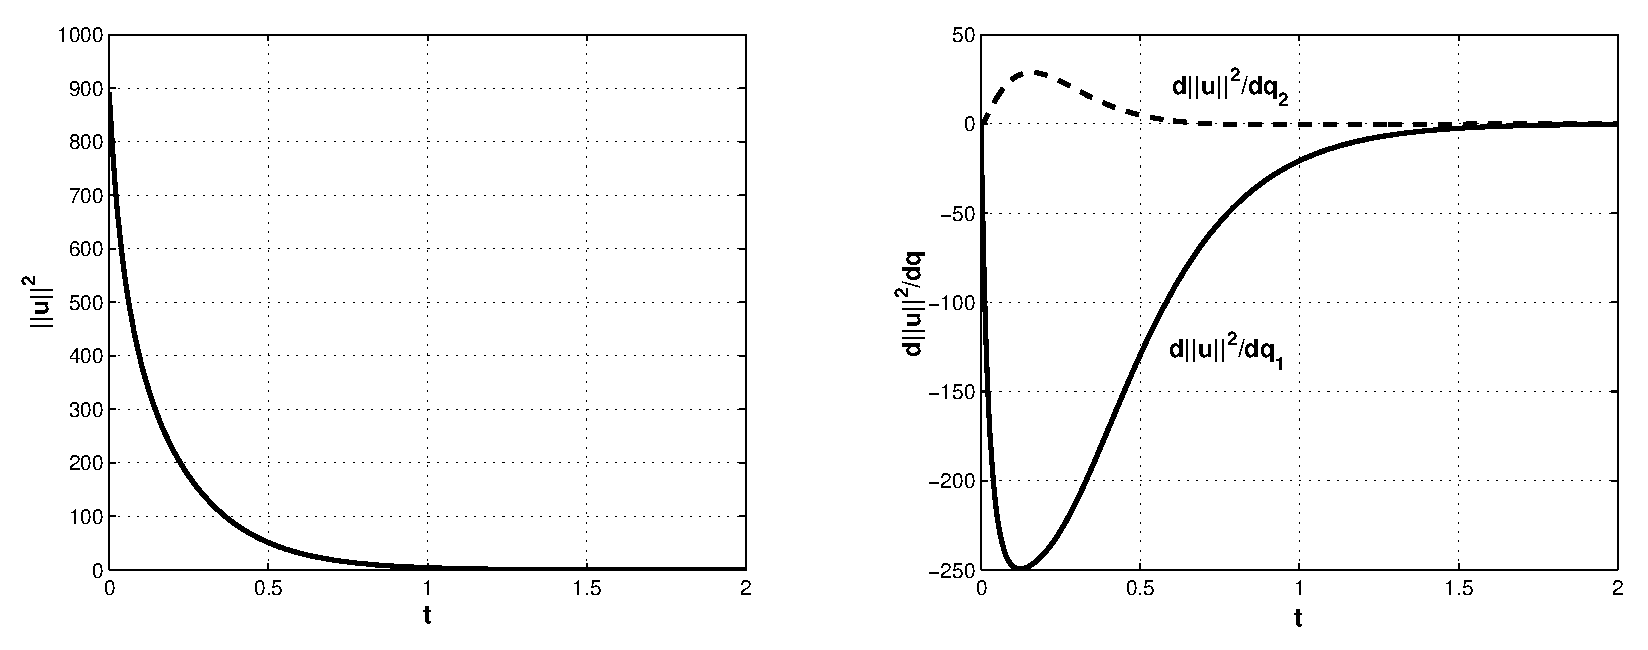
\epsfig{file=cvsfwdnonx.eps,width=\textwidth}}}
  \caption{Results for the \id{cvsAdvDiff\_FSA\_non} example problem.
    The time evolution of the squared solution norm, $||u||^2$, is shown on the left. 
    The figure on the right shows the evolution of the sensitivities of $||u||^2$
    with respect to the two problem parameters.}
  \label{f:cvsAdvDiff_FSA_non}
\end{figure}
%%
The output generated by \id{cvsAdvDiff\_FSA\_non} when computing
sensitivities with the \id{CV\_SIMULTANEOUS} method and full error
control (\id{cvsAdvDiff\_FSA\_non -sensi sim t}) is as follows:

\includeOutput{cvsAdvDiff\_FSA\_non}{../../examples/cvodes/serial/cvsAdvDiff_FSA_non.out}

%--------------------------------------------------------------------

\subsection{A serial dense example: cvsRoberts\_FSA\_dns}
\label{ss:cvsRoberts_FSA_dns}

This example is a modification of the chemical kinetics example \id{cvRoberts\_dns}
described in~\cite{cvode_ex}.  It computes, in addition to the solution of the
IVP, sensitivities of the solution with respect to the three reaction rates 
involved in the model. The ODEs are written as:
\begin{equation}\label{e:cvsRoberts_FSA_dns_ode}
  \begin{split}
    {\dot y}_1 &= -p_1 y_1 + p_2 y_2 y_3   \\
    {\dot y}_2 &=  p_1 y_1 - p_2 y_2 y_3 - p_3 y_2^2 \\
    {\dot y}_3 &=  p_3 y_2^2 \, ,
  \end{split}
\end{equation}
with initial conditions at $t_0 = 0$, $y_1 = 1$ and $y_2 = y_3 = 0$. 
The nominal values of the reaction rate constants are 
$p_1 = 0.04$, $p_2 = 10^4$ and $p_3 = 3\cdot 10^7$.
The sensitivity systems that are solved together with (\ref{e:cvsRoberts_FSA_dns_ode}) are
\begin{equation}\label{e:cvsRoberts_FSA_dns_sens}
  \begin{split}
    & {\dot s}_i = 
    \begin{bmatrix}
      - p_1 &   p_2 y_3             &   p_2 y_2 \\
        p_1 & - p_2 y_3 - 2 p_3 y_2 & - p_2 y_2 \\
        0   &             2 p_3 y_2 &  0              
    \end{bmatrix}
    s_i + \frac{\partial f}{\partial p_i} ~,
    \quad s_i(t_0) = \begin{bmatrix} 0 \\ 0 \\ 0 \end{bmatrix}  ~,
    \quad i = 1,2,3 \\
    & \frac{\partial f}{\partial p_1} = \begin{bmatrix} -y_1 \\ y_1 \\ 0 \end{bmatrix}, \quad
    \frac{\partial f}{\partial p_2} = \begin{bmatrix} y_2 y_3 \\ -y_2 y_3 \\ 0 \end{bmatrix}, \quad
    \frac{\partial f}{\partial p_3} = \begin{bmatrix} 0 \\ - y_2^2 \\ y_2^2 \end{bmatrix} \, .
  \end{split}
\end{equation}

The main program is described below with emphasis on the sensitivity related components. 
These explanations, together with those given for the code \id{cvRoberts\_dns}
in~\cite{cvode_ex}, will also provide the user with a template for instrumenting 
an existing simulation code to perform forward sensitivity analysis.
As will be seen from this example, an existing simulation code can be modified to compute 
sensitivity variables (in addition to state variables) by only inserting a few {\cvodes} 
calls into the main program. 

First note that no new header files need be included. In addition to the constants already
defined in \id{cvRoberts\_dns}, we define the number of model parameters, \id{NP} ($=3$),
the number of sensitivity parameters, \id{NS} ($=3$), and a constant \id{ZERO} $=0.0$. 

As mentioned in \ugref{s:forward_usage}, the user data structure \id{data}
must provide access to the array of model parameters as the only way for
{\cvodes} to communicate parameter values to the right-hand side function
\id{f}. In the \id{cvsRoberts\_FSA\_dns} example this is done by defining
\id{data} to be of type \id{UserData}, i.e. a pointer to a structure which contains
an array of \id{NP} \id{realtype} values.

Four user-supplied functions are defined. The function \id{f}, passed to \id{CVodeInit},
computes the right-hand side of the ODE (\ref{e:cvsRoberts_FSA_dns_ode}), while
\id{Jac} computes the dense Jacobian of the problem and is attached to the
dense linear solver module {\cvdense} through a call to \id{CVDlsSetDenseJacFn}.
The function \id{fS} computes the right-hand side of each sensitivity system
(\ref{e:cvsRoberts_FSA_dns_sens}) for one parameter at a time and is therefore of type
\id{SensRhs1}. Finally, the function \id{ewt} computes the error weights for the WRMS norm
estimations within {\cvodes}.

The program prologue ends by defining six private helper functions.  The first two,
\id{ProcessArgs} and \id{WrongArgs} (which would not be present in a typical user code),
parse and verify the command line arguments to \id{cvsRoberts\_FSA\_dns}, respectively.
After each successful return from the main {\cvodes} integrator, the functions 
\id{PrintOutput} and \id{PrintOutputS} print the state and sensitivity variables,
respectively. The function \id{PrintFinalStats} is called after completion of the
integration to print solver statistics.
The function \id{check\_flag} is used to check the return flag from any of the
{\cvodes} interface functions called by \id{main}.

The \id{main} program begins with definitions and type declarations. 
Among these, it defines the vector \id{pbar} of \id{NS} scaling factors for
the model parameters \id{p}, and the array \id{yS} of vectors (of type \id{N\_Vector})
which will contain the initial conditions and solutions for the sensitivity
variables. It also declares the variable \id{data} of type \id{UserData} 
which will contain the user-defined data structure to be passed to
{\cvodes} and used in the evaluation of the ODE right-hand sides.

The first code block in \id{main} deals with reading and interpreting
the command line arguments. \id{cvsRoberts\_FSA\_dns} can be run with
or without sensitivity computations turned on and with different
selections for the sensitivity method and error control strategy.

The user's data structure is then allocated and its field {\em p} is set to contain
the values of the three problem parameters.
%%
The next block of code is identical to that in \id{cvRoberts\_dns.c} (see \cite{cvode_ex})
and involves allocation and initialization of the state variables, and creation and 
initialization of \id{cvode\_mem}, the {\cvodes} solver memory. It specifies that
a user-provided function (\id{ewt}) is to be used for computing the error weights.
It also attaches {\cvdense}, with a non-\id{NULL} Jacobian function, as the linear solver 
to be used in the Newton nonlinear iteration.

If sensitivity analysis is enabled (through the command line arguments), 
the main program will then set the scaling parameters
\id{pbar} (\id{pbar}$_i$ = \id{p}$_i$, which can typically be used for 
nonzero model parameters). 
Next, the program allocates memory for \id{yS}, by calling the {\nvecs} function 
\id{N\_VCloneVectorArray\_Serial}, and initializaes all sensitivity variables to $0.0$.

The call to \id{CVodeSensInit1} specifies the sensitivity solution
method through the argument \id{sensi\_meth} (read from the command
line arguments) as one of \id{CV\_SIMULTANEOUS}, \id{CV\_STAGGERED},
or \id{CV\_STAGGERED1}.  It also specifies the user-defined routine, \id{fS},
for evaluation of the right-hand sides of sensitivity equations.

The next three calls specify optional inputs for forward sensitivity analysis:
specifying that sensitivity tolerances are to be based on \id{pbar},
the error control strategy (read from the command line arguments), and
the information on the model parameters.
In this example, only \id{pbar} is needed for the estimation of absolute sensitivity
variable tolerances; neither \id{p} nor \id{plist} is required since the
sensitivity right-hand sides are computed in the user function \id{fS}.  As a consequence,
we pass \id{NULL} for the corresponding arguments in \id{CVodeSetSensParams}.

Note that this example uses the default estimates for the relative and absolute tolerances 
\id{rtolS} and \id{atolS} for sensitivity variables, based on the tolerances for state 
variables and the scaling parameters \id{pbar} (see \ugref{ss:fwd_sensi} for details).

Next, in a loop over the \id{NOUT} output times, the program calls the integration
routine \id{CVode} which, if sensitivity analysis was initialized through the call
to \id{CVodeSensInit1}, computes both state and sensitivity variables. However,
\id{CVode} returns only the state solution at \id{tout} in the vector \id{y}.
The program tests the return from \id{CVode} for a value other than \id{CV\_SUCCESS} and
prints the state variables.
Sensitivity variables at \id{tout} are loaded into \id{yS} by calling \id{CVodeGetSens}.
The program tests the return from \id{CVodeGetSens} for a value other than \id{CV\_SUCCESS} 
and then prints the sensitivity variables.

Finally, the program prints some statistics (function \id{PrintFinalStats}) 
and deallocates memory through calls
to \id{N\_VDestroy\_Serial}, \id{N\_VDestroyVectorArray\_Serial}, 
\id{CVodeFree}, and \id{free} for the user data structure.

The user-supplied functions \id{f} (for the right-hand side of the original ODEs) and
\id{Jac} (for the system Jacobian) are identical to those in \id{cvRoberts\_dns.c},
with the notable exeption that model parameters are extracted from the user-defined
data structure \id{data}, which must first be cast to the \id{UserData} type.
Similarly, the user-supplied function \id{ewt} is identical to that in
\id{cvRoberts\_dns\_uw.c}.  The user-supplied function \id{fS} computes the
sensitivity right-hand side for the \id{iS}-th sensitivity equation.

Results generated by \id{cvsRoberts\_FSA\_dns} are shown in
Fig.~\ref{f:cvsRoberts_FSA_dns}. 
%%
\begin{figure}
  {\centerline{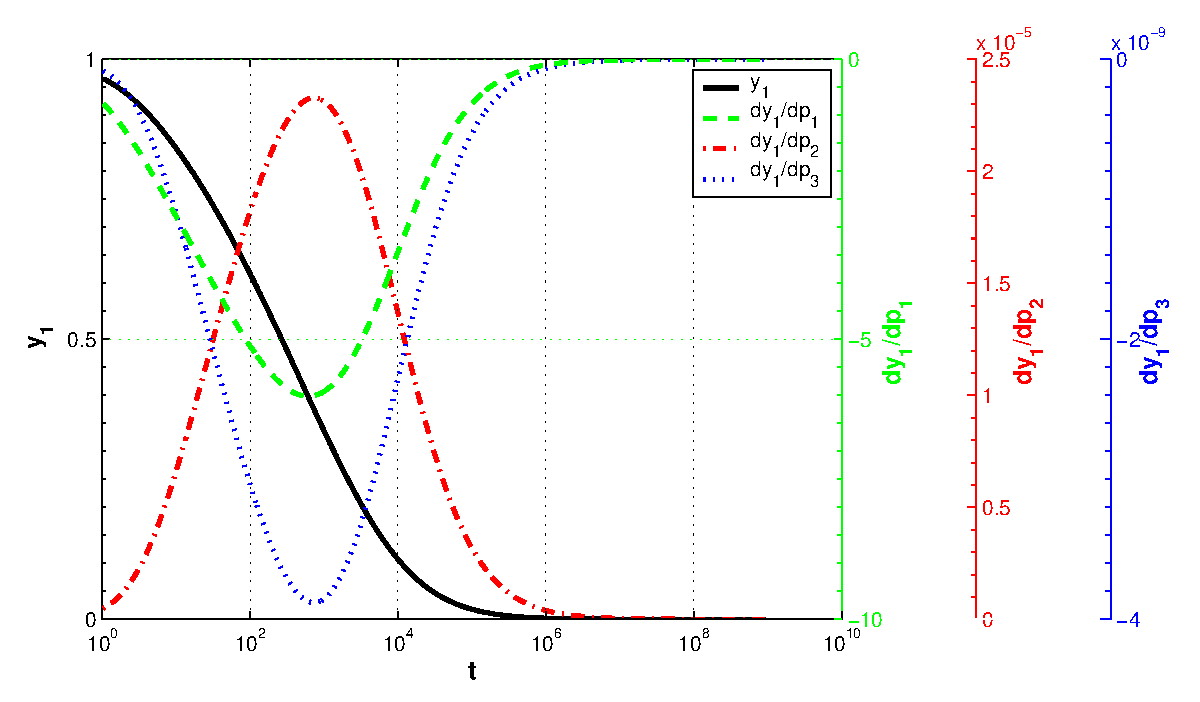
\epsfig{file=cvsfwddenx.eps,width=\textwidth}}}
  \caption{Results for the \id{cvsRoberts\_FSA\_dns} example problem:
    time evolution of $y_1$ and its sensitivities with respect to the
    three problem parameters.  (Note the four different vertical scales.)}
  \label{f:cvsRoberts_FSA_dns}
\end{figure}
%%
The following output is generated by \id{cvsRoberts\_FSA\_dns} when computing
sensitivities with the \id{CV\_SIMULTANEOUS} method and full error
control (\id{cvsRoberts\_FSA\_dns -sensi sim t}):

\includeOutput{cvsRoberts\_FSA\_dns}{../../examples/cvodes/serial/cvsRoberts_FSA_dns.out}


%----------------------------------------------------------------------------------

\subsection{A parallel example with user preconditioner: cvsDiurnal\_FSA\_kry\_p}
\label{ss:cvsDiurnal_FSA_kry_p}

As an example of using the forward sensitivity capabilities in {\cvodes} 
with the Krylov linear solver {\cvspgmr} and the {\nvecp} module, we describe
a test problem (derived from \id{cvDiurnal\_kry\_p}) that solves the
semi-discrete form of a two-species diurnal kinetics advection-diffusion PDE 
system in 2-D space, for which we also compute solution sensitivities with respect to 
problem parameters ($q_1$ and $q_2$) that appear in the kinetic rate terms.

The PDE system is
%%
\begin{equation}\label{e:cvsDiurnal_FSA_kry_p_PDE}
  \frac{\partial c^i}{\partial t} = K_h\frac{\partial^2 c^i}{\partial x^2}
  +V \frac{\partial c^i}{\partial x}
  + \frac{\partial} {\partial y} K_v(y) \frac{\partial c^i}{\partial y}
  + R^i(c^1,c^2,t) \quad (i=1,2) \, ,
\end{equation}
where the superscripts $i$ are used to distinguish the two chemical
species, and where the reaction terms are given by
\begin{equation}\label{e:cvsDiurnal_FSA_kry_p_R}
  \begin{split}
    R^1(c^1,c^2,t) & = -q_1c^1c^3-q_2c^1c^2+2q_3(t)c^3+q_4(t)c^2 ~, \\
    R^2(c^1,c^2,t) & = q_1c^1c^3-q_2c^1c^2-q_4(t)c^2 ~.
  \end{split}
\end{equation}
The spatial domain is $0 \leq x \leq 20,\;30 \leq y \leq 50$ (in {\em km}). 
The various constants and parameters are: $K_h=4.0\cdot 10^{-6},
~ V=10^{-3},~ K_v=10^{-8}\exp (y/5),~ q_1=1.63\cdot 10^{-16},
~ q_2=4.66\cdot 10^{-16},~ c^3=3.7\cdot 10^{16},$ and the diurnal
rate constants are defined as:
\begin{equation*}
  q_i(t) = 
  \left\{ \begin{array}{ll}
      \exp [-a_i/\sin \omega t], & \mbox{for } \sin \omega t>0 \\
      0, & \mbox{for } \sin \omega t\leq 0
    \end{array} \right\} ~~~(i=3,4) \, ,
\end{equation*}
where $\omega =\pi /43200, ~ a_3=22.62,~ a_4=7.601.$  The time interval of
integration is $[0, 86400]$, representing 24 hours measured in seconds.

Homogeneous Neumann boundary conditions are imposed on each boundary, and the
initial conditions are 
\begin{equation} \label{e:cvsDiurnal_FSA_kry_p_IC}
  \begin{split}
  c^{1}(x,y,0) &= 10^{6}\alpha (x)\beta (y) ~,~~~ 
                    c^{2}(x,y,0)=10^{12}\alpha(x)\beta (y) ~, \\
  \alpha (x) &= 1-(0.1x-1)^{2}+(0.1x-1)^{4}/2 ~, \\
  \beta (y) &= 1-(0.1y-4)^{2}+(0.1y-4)^{4}/2 ~.
  \end{split} 
\end{equation}
%%
We discretize the PDE system with central differencing, to
obtain an ODE system ${\dot u} = f(t,u)$ representing (\ref{e:cvsDiurnal_FSA_kry_p_PDE}).  
In this case, the discrete solution vector is distributed across
many processes.  Specifically, we may think of the processes as
being laid out in a rectangle, and each process being assigned a
subgrid of size \id{MXSUB}$\times$\id{MYSUB} of the $x-y$ grid. If
there are \id{NPEX} processes in the $x$ direction and \id{NPEY}
processes in the $y$ direction, then the overall grid size is
\id{MX}$\times$\id{MY} with \id{MX}$=$\id{NPEX}$\times$\id{MXSUB} and
\id{MY}$=$\id{NPEY}$\times$\id{MYSUB}, and the size of the ODE system is
$2\cdot$\id{MX}$\cdot$\id{MY}.  

To compute $f$ in this setting, the processes pass and receive
information as follows.  The solution components for the bottom row of
grid points assigned to the current process are passed to the process below
it, and the solution for the top row of grid points is received from
the process below the current process. The solution for the top
row of grid points for the current process is sent to the process
above the current process, while the solution for the bottom row of
grid points is received from that process by the current
process. Similarly, the solution for the first column of grid points
is sent from the current process to the process to its left, and
the last column of grid points is received from that process by the
current process. The communication for the solution at the right
edge of the process is similar. If this is the last process in a
particular direction, then message passing and receiving are bypassed
for that direction.

The overall structure of \id{main} is very
similar to that of the code \id{cvsRoberts\_FSA\_dns} described above, with 
differences arising from the use of the parallel {\nvector} module, {\nvecp}.
On the other hand, the user-supplied routines in \id{cvsDiurnal\_FSA\_kry\_p},
\id{f} for the right-hand side of the original system,
\id{Precond} for the preconditioner setup, and \id{PSolve} for the
preconditioner solve, are identical to those defined in the example program
\id{cvDiurnal\_kry\_p} described in \cite{cvode_ex}. The only difference is in the
routine \id{fcalc}, which operates on local data only and contains the actual 
calculation of $f(t,u)$, where the problem parameters are first extracted from the
user data structure \id{data}. The program \id{cvsDiurnal\_FSA\_kry\_p} defines no
additional user-supplied routines, as it uses the {\cvodes} internal difference quotient
routines to compute the sensitivity equation right-hand sides.

Sample results generated by \id{cvsDiurnal\_FSA\_kry\_p} are shown in
Fig.~\ref{f:cvsDiurnal_FSA_kry_p}. 
These results were generated on a $(2\cdot40)\times(2\cdot40)$ spatial grid.
%%
\begin{figure}
  {\centerline{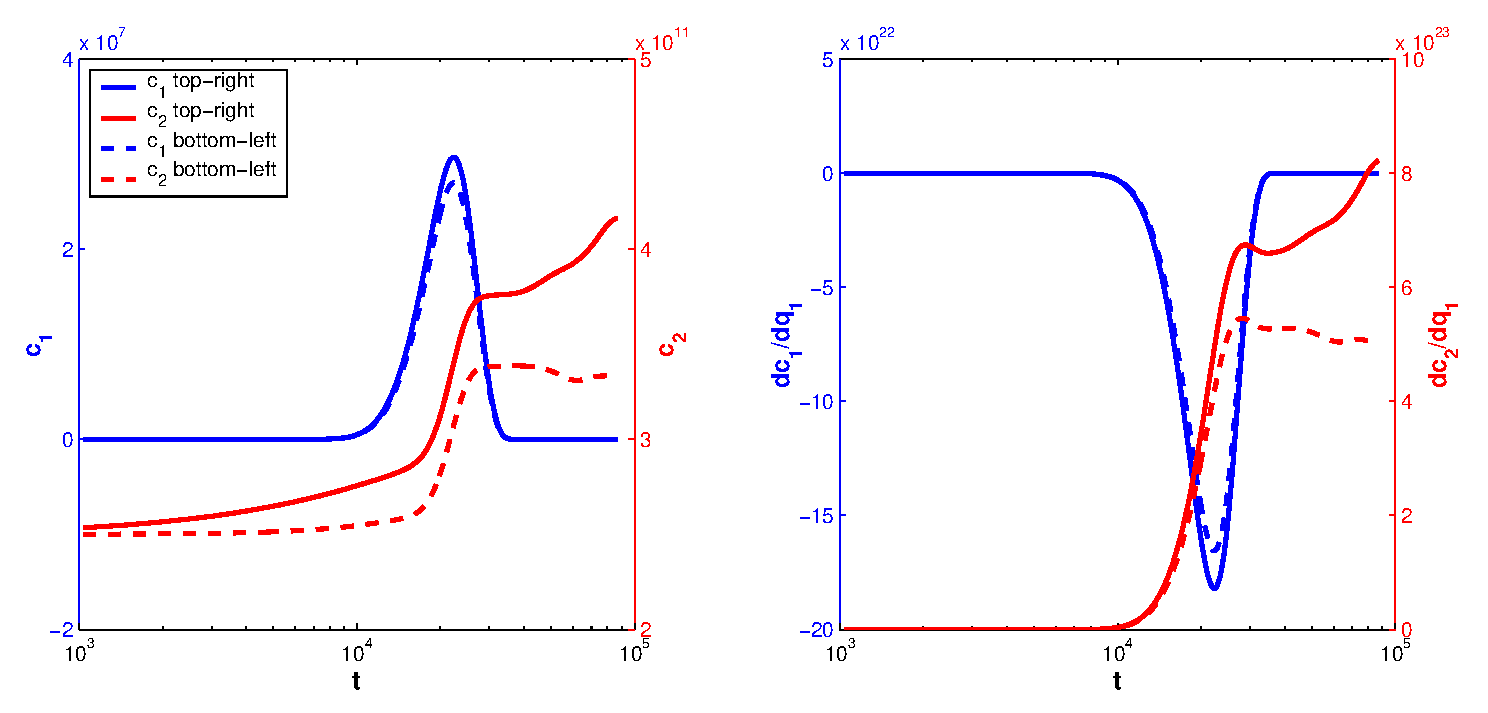
\epsfig{file=cvsfwdkryx_p.eps,width=\textwidth}}}
  \caption{Results for the \id{cvsDiurnal\_FSA\_kry\_p} example problem:
    time evolution of $c_1$ and $c_2$ at the bottom-left and top-right corners
    (left) and of their sensitivities with respect to $q_1$.}
  \label{f:cvsDiurnal_FSA_kry_p}
\end{figure}
%%
The following output is generated by \id{cvsDiurnal\_FSA\_kry\_p} when computing
sensitivities with the \id{CV\_SIMULTANEOUS} method and full error
control (\id{mpirun -np 4 cvsDiurnal\_FSA\_kry\_p -sensi sim t}):

\includeOutput{cvsDiurnal\_FSA\_kry\_p}{../../examples/cvodes/parallel/cvsDiurnal_FSA_kry_p.out}
